\documentclass[12pt]{article}
\usepackage[utf8x]{inputenc}
\usepackage[russian]{babel}
%%%%%%%%%%%%%%%%%%%%%%%%%%%%%%%%%%%%%%%%%%%%%%%%%%%%%%%%%%%%%%%%%%%%%%%%%%%%%%%%%%%%%%%%%%%%%%%%%%%%
\usepackage{amsmath,amssymb,amsthm}
\usepackage{color}
\usepackage{graphicx}
\usepackage{ucs}
\usepackage[unicode,verbose]{hyperref}


\newtheorem{statement}{Утверждение}
\newtheorem{theorem}{Теорема}
\newtheorem{corollary}{Следствие}[theorem]
\newtheorem{lemma}{Лемма}
\newtheorem{mynote}{Замечание}[section]
\theoremstyle{definition}
\newtheorem{definition}{Определение}
\newtheorem{remark}{Ремарка}
\newtheorem{example}{Пример}
\newcommand{\go}{\stackrel{\circ }{\mathfrak{g}}}
\newcommand{\ao}{\stackrel{\circ }{\mathfrak{a}}}
\newcommand{\co}[1]{\stackrel{\circ }{#1}}
\newcommand{\pia}{\pi_{\mathfrak{a}}}
\newcommand{\piab}{\pi_{\mathfrak{a}_{\bot}}}
\newcommand{\gf}{\mathfrak{g}}
\newcommand{\af}{\mathfrak{a}}
\newcommand{\aft}{\widetilde{\mathfrak{a}}}
\newcommand{\afb}{\mathfrak{a}_{\bot}}
\newcommand{\hf}{\mathfrak{h}}
\newcommand{\hfb}{\mathfrak{h}_{\bot}}
\newcommand{\pf}{\mathfrak{p}}
%\input{tcilatex}

\begin{document}

\title{Рекурсивные свойства ветвления и БГГ резольвента}
\author{В Д Ляховский$^1$, А А Назаров$^2$\\
Теоретический отдел,\\ Санкт - Петербургский государственный университет\\
198904, Санкт - Петербург, Россия\\
$^1$e-mail: lyakh1507@nm.ru, $^2$ antonnaz@gmail.com}

\maketitle

\begin{abstract}
Рекуррентные соотношения для коэффициентов ветвления основываются на определенном разложении сингулярного элемента. Мы показываем, что такое разложение может использоваться для построения параболических модулей Верма и получения обобщенных формул Вейля-Верма для характеров. Также мы демонстрируем, что коэффициенты ветвления определяют обобщенную резольвенту Бернштейна-Гельфанда-Гельфанда. 
\end{abstract}


\section{Введение}

\label{sec:introduction}
Свойства ветвления (аффинных) алгебр Ли важны для приложений в квантовой теории поля (смотри, например, модели конформной теории поля \cite{difrancesco1997cft},\cite{coquereaux2008conformal}). В данной работе мы показываем, что ветвление для произвольной редуктивной подалгебры связано с БГГ резольвентой и проявляет свойства резольвенты в категории $\mathcal{O}^{p}$ \cite{lepowsky1977generalization} (параболического обобщения категории $\mathcal{O}$ \cite{bernstein1976category}).

Резольвента для неприводимых модулей в терминах бесконечномерных модулей важна для теории интегрируемых спиновых цепочек \cite{derk1008}. В подходе  $\mathcal{Q}$-оператора Бакстера \cite{derk09} общие трансфер-матрицы, соответствующие (обобщенным) модулям Верма, факторизуются в произведение операторов Бакстера. Резольвента позволяет вычислить трансфер-матрицы для конечномерных вспомогательных пространств.

Чтобы продемонстрировать связь БГГ резольвенты с ветвлением мы используем рекурсивный подход, представленный в работе \cite
{2010arXiv1007.0318L} (похожий подход для максимальных вложений использовался в работе \cite{ilyin812pbc}). Мы рассматриваем подалгебру $\af \hookrightarrow \gf$ вместе с $\afb$ -- ``ортогональным партнером'' $\af$ по отношению к форме Киллинга, а также  $\widetilde{\afb}:=\afb\oplus \frak{h}_{\perp }$, где $\frak{h}=\frak{\frak{h}_{\af}}\oplus
\frak{h}_{\afb}\oplus \frak{h}_{\perp }$. Для любой редуктивной подалгебры $\af$ подалгебра $\afb\hookrightarrow \gf$ регулярна и редуктивна. Для интегрируемого модуля старшего веса $%
L^{\left(\mu \right) }$ и ортогональной подалгебры  $\af_{\bot }$ мы рассматриваем сингулярный элемент $\Psi ^{\left( \mu \right) }$ (числитель в формуле Вейля для характеров $ch\left( L^{\mu }\right) =\frac{\Psi ^{\left(
\mu \right) }}{\Psi ^{\left( 0\right) }}$, см., например,  \cite
{humphreys1997introduction}) и знаменатель Вейля $\Psi _{\af_{\bot
  }}^{\left( 0\right) }$ для ортогонального партнера. В работе показано, что элемент  $\Psi _{\gf%
}^{\left( \mu \right) }$ может быть разложен в комбинацию числителей Вейля $\Psi _{\af_{\bot }}^{\left( \nu \right) }$, где $\nu \in P_{%
\mathfrak{a}_{\bot}}^{+}$. Это разложение дает возможность построить множество модулей старшего веса $L_{\afb}%
^{\mu _{\afb}}$. В том случае, если вложение\ $\af%
_{\bot }\hookrightarrow \gf$ \ удовлетворяет ``стандартным параболическим'' условиям, эти модули порождают параболические модули Верма $M_{\left(
\afb \hookrightarrow \gf\right) }^{\mu _{%
\afb}}$, так что исходный характер $ch\left(
L^{\mu }\right) $ в итоге раскладывается в чередующуюся сумму таких модулей. С другой стороны, если параболическое условие нарушено, конструкция сохраняется и порождает разложение по отношению к набору обобщенных модулей Верма  $M_{\left( \widetilde{\frak{b}_{\perp }},\gf\right) }^{\mu _{%
\widetilde{\afb}}}$, где $%
\widetilde{\frak{b}_{\perp }}$ уже не является подалгеброй в $\gf$, а оказывается сжатием $\widetilde{\afb}$.

Некоторые общие свойства предложенного разложения формулируются в терминах определенного формального элемента $\Gamma _{\af\rightarrow \gf}$, называемого ``веером вложения''. Использование этого инструмента позволило сформулировать простой и явный алгоритм для вычисления правил ветвления, подходящий для произвольной (максимальной или не максимальной) подалгебры в аффинной алгебре Ли \cite{2010arXiv1007.0318L}.

Возможные обобщения полученных результатов обсуждаются в Разделе \ref{sec:conclusions}.

\subsection{Обозначения}

\label{sec:notation}
Пусть $\frak{g}$ и $\frak{a}$ -- (аффинные) алгебры Ли, а вложение  $\frak{a}\hookrightarrow \frak{g}$ таково, что  $\frak{a}$ -- редуктивная подалгебра в  $\frak{a\subset g}$ с согласованным корневым пространством: $\frak{%
h}_{\frak{a}}^{\ast }\subset \frak{h}_{\frak{g}}^{\ast }$. Мы используем следующие обозначения:

$\frak{g=n}^{-}+\frak{h}+\frak{n}^{+}$ --- разложение Картана;

$r$ , $\left( r_{\frak{a}}\right) $ --- ранг алгебра $\frak{g}$ $%
\left( \mathrm{\text{соотв., }\frak{a}}\right) $ ;

$\Delta $ $\left( \Delta _{\frak{a}}\right) $--- корневая система; $\Delta
^{+} $ $\left( \mathrm{\text{соотв., }\Delta _{\frak{a}}^{+}}\right) $--- набор положительных корней (алгебр $\frak{g}$ и $\frak{a}$ соответственно);

$\mathrm{mult}\left( \alpha \right) $ $\left( \mathrm{mult}_{\frak{a}}\left(
\alpha \right) \right) $ --- кратность корня $\alpha$ в $%
\Delta $ (соотв., в $\left( \Delta _{\frak{a}}\right) $);

$S\quad \left( S_{\frak{a}}\right) $ --- множество простых корней (для 
$\gf$ и $\af$ соответственно);

$\alpha _{i}$ , $\left( \alpha _{\left( \frak{a}\right) j}\right) $ ---  $%
i$-й (соотв., $j$-й) простой корень алгебры $\frak{g}$ $\left( \mathrm{\text{соотв.,}\frak{a%
}}\right) $; $i=0,\ldots ,r$,\ \ $\left( j=0,\ldots ,r_{\frak{a}}\right) $;


$\alpha _{i}^{\vee }$ , $\left( \alpha _{\left( \frak{a}\right) j}^{\vee
}\right) $-- простой ко-корень для $\frak{g}$ $\left( \mathrm{\text{соотв.,}\frak{a}%
}\right) $ , $i=0,\ldots ,r$ ;\ \ $\left( j=0,\ldots ,r_{\frak{a}}\right) $;

$W$ , $\left( W_{\frak{a}}\right) $--- группа Вейля;

$C$ , $\left( C_{\frak{a}}\right) $--- фундаментальная камера Вейля;

$\bar{C}, \left(\bar{C_{\frak{a}}}\right)$ --- замыкание фундаментальной камеры Вейля;

$\epsilon \left( w\right) :=\left( -1\right) ^{\mathrm{length}(w)}$;

$\rho $\ , $\left( \rho _{\frak{a}}\right) $\ --- вектор Вейля;

$L^{\mu }$\ $\left( L_{\frak{a}}^{\nu }\right) $\ --- интегрируемый модуль  $\frak{g}$ со старшим весом $\mu $\ ; (соотв., интегрируемый $\af$-модуль старшего веса $\nu $);

$\mathcal{N}^{\mu }$ , $\left( \mathcal{N}_{\frak{a}}^{\nu }\right) $ ---
весовая диаграмма модуля $L^{\mu }$ (соотв., ${}L_{\frak{a}}^{\nu }$ );

$P$ (соотв., $P_{\frak{a}} $) \ --- весовая решетка;

$P^{+}$ (соотв., $P_{\frak{a}}^{+} $) \ --- решетка доминантных весов;

$m_{\xi }^{\left( \mu \right) }$ , $\left( m_{\zeta }^{\left( \nu \right)
}\right) $ --- кратность веса $\xi \in P$ \ $\left( \mathrm{\text{соотв., }\in P_{\frak{a}}}\right) $ в $L^{\mu }$, (соотв., в $\zeta \in
L_{\frak{a}}^{\nu } $);

$ch\left( L^{\mu }\right) $ (соотв., $\mathrm{ch}\left( L_{\frak{a}}^{\nu
}\right) $)--- формальный характер $L^{\mu }$ (соответственно, $L_{\frak{a}}^{\nu
} $);

$ch\left( L^{\mu }\right) =\frac{\sum_{w\in W}\epsilon (w)e^{w\circ (\mu
+\rho )-\rho }}{\prod_{\alpha \in \Delta ^{+}}\left( 1-e^{-\alpha }\right) ^{%
\mathrm{{mult}\left( \alpha \right) }}}$ --- формула Вейля-Каца;

$R:=\prod_{\alpha \in \Delta ^{+}}\left( 1-e^{-\alpha }\right) ^{\mathrm{{%
mult}\left( \alpha \right) }}\quad $ (соотв., $R_{\frak{a}}:=\prod_{\alpha \in
\Delta _{\frak{a}}^{+}}\left( 1-e^{-\alpha }\right) ^{\mathrm{mult}_{\frak{a}%
}\left( \alpha \right) } $)--- знаменатель Вейля.

\section{Ортогональная подалгебра и сингулярные элементы}

\label{sec:recurr-form-branch}

В этом разделе мы покажем, как рекуррентный подход к проблеме ветвления естественным образом приводит к представлению формального характера $\frak{g}$-модуля в виде комбинации характеров, соответствующих параболическим (обобщенным) модулям Верма. Рассмотрим редуктивную алгебру Ли  $\frak{g}$ и ее редуктивную подалгебру $\frak{a}\subset \frak{g}$.
Пусть  $L^{\mu} $ -- интегрируемый модуль старшего веса алгебры  $\frak{g}$, $\mu \in P^{+}$.  Будем считать  $L^{\mu}$ полностью приводимым по отношению к подалгебре $\frak{a}$,
\begin{equation*}
L_{\frak{g}\downarrow \frak{a}}^{\mu }=\bigoplus\limits_{\nu \in P_{\frak{a}%
}^{+}}b_{\nu }^{\left( \mu \right) }L_{\frak{a}}^{\nu }.
\end{equation*}
Это разложение может быть записано в терминах формальных характеров с использованием оператора проекции  $\pi _{\frak{a}}$ (на весовое пространство $\frak{h_{a}}^{\ast }$):
\begin{equation}
\pi _{\frak{a}}ch\left( L^{\mu }\right) =\sum_{\nu \in P_{\frak{a}%
}^{+}}b_{\nu }^{(\mu )}ch\left( L_{\frak{a}}^{\nu }\right) .
\label{branching1}
\end{equation}
Для модуля  $L^{\mu }$ существует БГГ резольвента (см. \cite
{bernstein1976category,bernstein1975differential,bernstein1971structure} и
\cite{humphreys2008representations}). Все члены фильтрующей последовательности представляются суммами модулей Верма со старшими весами $\nu$, сильно связанными с $\mu$:
\begin{equation*}
\left\{ \nu \right\} =\left\{ w\left( \mu +\rho \right) -\rho |w\in
W\right\} .
\end{equation*}

\subsection{Ортогональная подалгебра}

Пусть  $\frak{h}_{\frak{a}}$ -- подалгебра Картана в  $\mathfrak{g}$. Для  $\mathfrak{a}\hookrightarrow \frak{g}$ введем ``ортогонального партнера''  $\mathfrak{a}_{\bot }\hookrightarrow \frak{g}$.

Рассмотрим корневое подпространство  $\frak{h}_{\perp \frak{a}}^{\ast }$, ортогональное к $\frak{a}$,
\begin{equation*}
\frak{h}_{\perp \frak{a}}^{\ast }:=\left\{ \eta \in \frak{h}^{\ast }|\forall
h\in \frak{h}_{\frak{a}};\eta \left( h\right) =0\right\} ,
\end{equation*}
и корни  $\frak{g}$ (соответственно, положительные корни)  ортогональные к $\frak{a}$,
\begin{eqnarray}
\Delta _{\frak{a}_{\perp }} &:&=\left\{ \beta \in \Delta _{\frak{g}}|\forall
h\in \frak{h}_{\frak{a}};\beta \left( h\right) =0\right\} ,
\label{delta a ort} \\
\Delta _{\frak{a}_{\perp }}^{+} &:&=\left\{ \beta ^{+}\in \Delta _{\frak{g}%
}^{+}|\forall h\in \frak{h}_{\frak{a}};\beta ^{+}\left( h\right) =0\right\} .
\notag
\end{eqnarray}
Обозначим через  $W_{\frak{a}_{\perp }}$ подгруппу  $W$, порожденную отражениями  $w_{\beta }$ с корнями  $\beta \in \Delta_{\frak{a}_{\perp}}^{+}$. Корневая подсистема  $\Delta _{\frak{a}_{\perp }}$ определяет подалгебру  $\frak{a}_{\perp }$, имеющую подалгебру Картана $\frak{h}_{\frak{a}_{\perp }}$. Пусть
\begin{equation*}
\frak{h}_{\perp }^{\ast }:=\left\{ \eta \in \frak{h}_{\perp \frak{a}}^{\ast
}|\forall h\in \frak{h}_{\frak{a}\oplus \frak{a}_{\perp }};\eta \left(
h\right) =0\right\}
\end{equation*}
и у  $\frak{g}$ есть подалгебры
\begin{eqnarray}
\widetilde{\frak{a}_{\perp }} :=\frak{a}_{\perp }\oplus \frak{h}_{\perp }
\qquad
\widetilde{\frak{a}} :=\frak{a}\oplus \frak{h}_{\perp }.
\end{eqnarray}
Заметим, что  $\mathfrak{a} \oplus \mathfrak{a}_{\bot}$ в общем случае не является подалгеброй в $\mathfrak{g}$.

Для подалгебр Картана имеет место разложение
\begin{equation}
\frak{h}=\frak{\frak{h}_{\frak{a}}}\oplus \frak{h}_{\frak{a}_{\perp }}\oplus
\frak{h}_{\perp }=\frak{\frak{h}_{\widetilde{\frak{a}}}}\oplus \frak{h}_{%
\frak{a}_{\perp }}=\frak{\frak{h}_{\widetilde{\frak{a}_{\perp }}}}\oplus
\frak{h}_{\frak{a}}.
\end{equation}
Рассмотрим векторы Вейля  $\rho _{\frak{a}}$ и $\rho _{\frak{a}_{\perp}} $, соответствующие  $\frak{a}$ и $\frak{a}_{\perp }$.
Введем так называемые ``дефекты'' вложения  $\mathcal{D}_{\frak{a}}$ и $\mathcal{D}_{\frak{a}_{\perp }}$:
\begin{equation}
\mathcal{D}_{\frak{a}}:=\rho _{\frak{a}}-\pi _{\frak{a}}\rho , \qquad
\mathcal{D}_{\frak{a}_{\perp }}:=\rho _{\frak{a}_{\perp }}-\pi _{\frak{a}%
_{\perp }}\rho .  \label{defect ort}
\end{equation}
Для  $\mu \in P^{+}$ рассмотрим связанные веса  $\left\{\left( w(\mu +\rho )-\rho \right) |w\in W\right\} $ и их проекции на $h_{\frak{a}_{\perp }}^{\ast }$, дополнительно сдвинутые на дефект $-\mathcal{D}_{\frak{a}_{\perp }}$:
\begin{equation*}
\mu _{\frak{a}_{\perp }}\left( w\right) :=\pi _{\frak{a}_{\perp }}\left[
w(\mu +\rho )-\rho \right] -\mathcal{D}_{\frak{a}_{\perp }},\quad w\in W.
\end{equation*}

Среди весов  $\left\{ \mu _{\frak{a}_{\perp
}}\left( w\right) |w\in W\right\} $ всегда можно выбрать те, которые попадают в фундаментальную камеру $\overline{C_{\frak{a}_{\perp }}}$. Пусть $U$ -- множество представителей $u$ классов  $W/W_{\frak{a}_{\perp }}$, таких что
\begin{equation}
U:=\left\{ u\in W|\quad \mu _{\frak{a}_{\perp }}\left( u\right) \in
\overline{C_{\frak{a}_{\perp }}}\right\} \quad .  \label{U-def}
\end{equation}
Тогда можно выделить подмножества:
\begin{equation}
\mu _{\widetilde{\mathfrak{a}}}\left( u\right) :=\pi _{\widetilde{%
\mathfrak{a}}}\left[ u(\mu +\rho )-\rho \right] +\mathcal{D}_{\frak{a}%
_{\perp }},\quad u\in U,  \label{mu-a}
\end{equation}
и
\begin{equation}
\mu _{\frak{a}_{\perp }}\left( u\right) :=\pi _{\frak{a}_{\perp }}\left[
u(\mu +\rho )-\rho \right] -\mathcal{D}_{\frak{a}_{\perp }},\quad u\in U.
\label{mu-a-tilda}
\end{equation}

Заметим, что подалгебра  $\mathfrak{a}_{\bot}$ по определению регулярна, так как она построена на подмножестве корней алгебры $\mathfrak{g}$.

Для интересующих нас модулей формула Вейля-Каца для  $\mathrm{ch}\left( L^{\mu }\right) $ может быть записана через сингулярные элементы \cite{humphreys1997introduction},
\begin{equation*}
\Psi ^{\left( \mu \right) }:=\sum\limits_{w\in W}\epsilon (w)e^{w(\mu +\rho
)-\rho },
\end{equation*}
а именно,
\begin{equation}
\mathrm{ch}\left( L^{\mu }\right) =\frac{\Psi ^{\left( \mu \right) }}{\Psi
^{\left( 0\right) }}=\frac{\Psi ^{\left( \mu \right) }}{R}.
\label{Weyl-Kac2}
\end{equation}
То же верно и для подмодулей $\mathrm{ch}\left( L_{\frak{a}}^{\nu
}\right) $ в формуле (\ref{branching1})
\begin{equation*}
\mathrm{ch}\left( L_{\frak{a}}^{\nu }\right) =\frac{\Psi _{\frak{a}}^{\left(
\nu \right) }}{\Psi _{\frak{a}}^{\left( 0\right) }}=\frac{\Psi _{\frak{a}%
}^{\left( \nu \right) }}{R_{\frak{a}}},
\end{equation*}
где
\begin{equation*}
\Psi _{\frak{a}}^{\left( \nu \right) }:=\sum\limits_{w\in W_{\frak{a}%
}}\epsilon (w)e^{w(\nu +\rho _{_{\frak{a}}})-\rho _{_{\frak{a}}}}.
\end{equation*}
Применяя формулу  (\ref{Weyl-Kac2}) к правилу ветвления  (\ref{branching1}) мы получаем соотношение, связывающее сингулярные элементы $\Psi ^{\left( \mu
\right) }$ и $\Psi _{\frak{a}}^{\left( \nu \right) }$ :
\begin{eqnarray}
\pi _{\frak{a}}\left( \frac{\sum_{w \in W}\epsilon (w )e^{w (\mu +\rho
)-\rho }}{\prod_{\alpha \in \Delta ^{+}}(1-e^{-\alpha })^{\mathrm{mult}%
(\alpha )}}\right) &=&\sum_{\nu \in P_{\frak{a}}^{+}}b_{\nu }^{(\mu )}\frac{%
\sum_{w \in W_{\frak{a}}}\epsilon (w )e^{w (\nu +\rho _{\frak{a}})-\rho _{%
\frak{a}}}}{\prod_{\beta \in \Delta _{\frak{a}}^{+}}(1-e^{-\beta })^{\mathrm{%
mult}_{\frak{a}}(\beta )}},  \notag  \label{eq:4} \\
\pi _{\frak{a}}\left( \frac{\Psi ^{\left( \mu \right) }}{R}\right)
&=&\sum_{\nu \in P_{\frak{a}}^{+}}b_{\nu }^{(\mu )}\frac{\Psi _{\frak{a}%
}^{\left( \nu \right) }}{R_{\frak{a}}}.
\end{eqnarray}

\subsection{Разложение сингулярного элемента.}

\label{subsec:decomp-sing-element}

Теперь мы выполним разложение сингулярного элемента  $\Psi ^{\left(\mu \right) }$ на сингулярные элементы модулей ортогонального партнера:

\begin{lemma}

Пусть  $\frak{a}_{\bot }$ -- ортогональный партнер редуктивной подалгебры  $\frak{a}\hookrightarrow \frak{g}$ и $\frak{h}=\frak{\frak{h}_{\frak{a}}}\oplus \frak{h}_{\frak{a}_{\perp }}\oplus \frak{h}_{\perp }$, $\widetilde{%
\frak{a}_{\perp }}=\frak{a}_{\perp }\oplus \frak{h}_{\perp }$, $%
\widetilde{\frak{a}}=\frak{a}\oplus \frak{h}_{\perp }$.

Пусть $L^{\mu }$ -- интегрируемый модуль старшего веса  $\mu \in P^{+}$ и 

$\Psi ^{\left( \mu \right) }$\ -- сингулярный элемент $L^{\mu }$.

Тогда элемент  $\Psi ^{\left( \mu \right) }$ может быть разложен в сумму по  $u\in U$ (см. (\ref{U-def})) сингулярных элементов $\Psi _{\frak{a}_{\perp }}^{\mu _{\frak{a}_{\perp }}\left( u\right) }$ с коэффициентами
$\epsilon (u)e^{\mu _{\widetilde{\mathfrak{a}}}\left( u\right) }$:
\begin{equation}
\Psi ^{\left( \mu \right) }=\sum_{u\in U}\;\epsilon (u)e^{\mu _{\widetilde{%
\mathfrak{a}}}\left( u\right) }\Psi _{\frak{a}_{\perp }}^{\mu _{\frak{a}%
_{\perp }}\left( u\right) }.  \label{sing decomp main}
\end{equation}
\label{Psi-decomp-lemma}
\end{lemma}

\begin{proof}
Пусть
\[
u(\mu +\rho )=\pi _{\left( \aft\right) }u(\mu +\rho )+\pi _{\left(
\frak{a}_{\perp }\right) }u(\mu +\rho ),
\]
где $u\in U$. Для произвольного  $v\in W_{\frak{a}_{\bot }}$ рассмотрим сингулярный вес  $vu(\mu +\rho )-\rho $ и выполним разложение:
\begin{equation}
\begin{array}{lcl}
vu(\mu +\rho )-\rho  & = & \pi _{\left( \frak{a}\right) }\left( u(\mu +\rho
)\right) -\rho +\rho _{\frak{a}_{\perp }}
\\
&  & +\ v\left( \pi _{\left( \aft_{\perp }\right) }u(\mu
+\rho )-\rho _{\frak{a}_{\perp }}+\rho _{\frak{a}_{\perp }}\right) -\rho _{%
\frak{a}_{\perp }} .
\end{array}
\label{sing-decomp-1}
\end{equation}
Используем дефект $\mathcal{D}_{\frak{a}_{\bot }}$ (\ref{defect ort}), чтобы упростить первую строчку в формуле (\ref{sing-decomp-1}):
\[
\begin{array}{r}
\pi _{\left( \aft\right) }\left( u(\mu +\rho )\right) -\rho +\rho _{%
\frak{a}_{\perp }}= \\
\pi _{\left( \aft\right) }\left( u(\mu +\rho )\right) -\pi _{\aft%
}\rho -\pi _{\af_{\bot }}\rho +\rho _{\frak{a}_{\bot }}= \\
=\pi _{\left( \aft\right) }\left( u(\mu +\rho )-\rho \right) +\mathcal{D}%
_{\frak{a}_{\bot }},
\end{array}
\]
и вторую
\[
\begin{array}{c}
v\left( \pi _{\left( \frak{a}_{\perp }\right) }u(\mu +\rho
)-\rho _{\frak{a}_{\perp }}+\rho _{\frak{a}_{\perp }}\right) -\rho _{\frak{a}%
_{\perp }}= \\
v\left( \pi _{\left( \frak{a}_{\bot }\right) }u(\mu +\rho )-%
\mathcal{D}_{\frak{a}_{\bot }}-\pi _{\left( \frak{a}_{\bot }\right) }\rho
+\rho _{\frak{a}_{\bot }}\right)
-\rho _{\frak{a}_{\bot }}= \\
=v\left( \pi _{\left( \frak{a}_{\bot }\right) }\left[ u(\mu
+\rho )-\rho \right] -\mathcal{D}_{\frak{a}_{\bot }}+\rho _{\frak{a}_{\bot
}}\right) -\rho _{\frak{a}_{\bot }}.
\end{array}
\]
В результате получаем требуемое разложение сингулярного элемента $\Psi ^{\mu }$ на сингулярные элементы $\Psi_{\frak{a}_{\perp}}^{\eta}$ модулей $L_{\frak{a}_{\perp }}^{\eta }$ подалгебры $\frak{a}_{\perp }$: 
\begin{equation}
\begin{array}{l}
\Psi ^{\mu }=\sum_{u\in U}\sum_{v\in W_{\frak{a}_{\perp }}}\epsilon
(v)\epsilon (u)e^{vu(\mu +\rho )-\rho }= \\
=\sum_{u\in U}\epsilon (u)e^{\pi _{\aft}\left[ u(\mu +\rho )-\rho \right]
+\mathcal{D}_{\frak{a}_{\perp }}}\sum_{v\in W_{\frak{a}_{\perp }}}\epsilon
(v)e^{v\left( \pi _{\left( \frak{a}_{\perp }\right) }\left[
u(\mu +\rho )-\rho \right] -\mathcal{D}_{\frak{a}_{\perp }}+\rho _{\frak{a}%
_{\perp }}\right) -\rho _{\frak{a}_{\perp }}}= \\
=\sum_{u\in U}\;\epsilon (u)\Psi _{\af_{\perp }}^{\pi
_{\left( \frak{a}_{\perp }\right) }\left[ u(\mu +\rho )-\rho
\right] -\mathcal{D}_{\frak{a}_{\perp }}}e^{\pi _{\left( \aft\right) }%
\left[ u(\mu +\rho )-\rho \right] +\mathcal{D}_{\frak{a}_{\perp }}}.
\end{array}
\label{singular main}
\end{equation}
\end{proof}

\bigskip

\begin{remark}
Это соотношение можно рассматривать как обобщенную форму формулы Вейля для сингулярного элемента $\Psi _{\frak{g}}^{\mu }$: векторы $\mu _{%
\widetilde{\mathfrak{a}}}\left( u\right) $ играют роль сингулярных весов, а чередующиеся множители  $\epsilon (u)$ расширены до $\epsilon
(u)\Psi _{\frak{a}_{\perp }}^{\mu _{\frak{a}_{\perp }}\left( u\right) }$.

Действительно, при  $\frak{a=g}$ подалгебры  $\frak{a}_{\perp }$, и $\frak{h}_{\perp }$ тривиальны, $U=W$ и оригинальная формула Вейля восстанавливается, так как сингулярные элементы $\epsilon (u)\Psi _{\frak{a}_{\perp %
}}^{\mu _{\frak{a}_{\perp }}\left( u\right) }=\epsilon (u)$ становятся  тривиальными.

В противоположном пределе, когда $\frak{a}=0$, $\Delta _{\frak{a}_{\perp }}=\Delta _{\frak{g}}$, $%
\frak{h}_{\perp }^{\ast }=0$, $\frak{a}_{\perp }=\frak{g}$, $\mathcal{D}_{%
\frak{a}_{\perp }}=0$ и $U=W/W_{\frak{a}_{\perp }}=e$, опять восстанавливается сингулярный элемент
 $\Psi ^{\mu }$, теперь в результате тривиализации множества векторов $\mu _{\af}\left( e\right) =0$.
\end{remark}

\begin{remark}

В работе \cite{2010arXiv1007.0318L} разложение, аналогичное формуле (\ref{singular main}) было использовано для построения рекуррентных соотношений для коэффициентов ветвления $k_{\xi}^{\left( \mu \right) }$, соответствующих вложению  $\frak{a}\hookrightarrow \frak{g}$:
\begin{equation}
\begin{array}{c}
k_{\xi }^{\left( \mu \right) }=-\frac{1}{s\left( \gamma _{0}\right) }\left(
\sum_{u\in U}\epsilon (u)\;\dim \left( L_{\frak{a}_{\perp }}^{\mu _{\frak{a}%
_{\perp }}\left( u\right) }\right) \delta _{\xi -\gamma _{0},\pi _{%
\widetilde{\frak{a}}}(u(\mu +\rho )-\rho )}+\right.  \\
\left. +\sum_{\gamma \in \Gamma _{\widetilde{\frak{a}}\rightarrow \frak{g}%
}}s\left( \gamma +\gamma _{0}\right) k_{\xi +\gamma }^{\left( \mu \right)
}\right) .
\end{array}
\label{recurrent rel}
\end{equation}
Рекурсия задается множеством  $\Gamma _{\widetilde{\frak{a}}\rightarrow \frak{g}}$, называемом веером вложения. Это множество определяется как носитель  $\left\{ \xi \right\}_{\frak{a}\rightarrow \frak{g}}$  коэффициентной функции $s(\xi )$
\begin{equation*}
\left\{ \xi \right\} _{\widetilde{\frak{a}}\rightarrow \frak{g}}:=\left\{
\xi \in P_{\widetilde{\frak{a}}}|s(\xi )\neq 0\right\},
\end{equation*}
возникающей в разложении 
\begin{equation}
\prod_{\alpha \in \Delta ^{+}\setminus \Delta _{\bot }^{+}}\left( 1-e^{-\pi
_{\widetilde{\frak{a}}}\alpha }\right) ^{\mathrm{mult}(\alpha )-\mathrm{mult}%
_{\frak{a}}(\pi _{\widetilde{\frak{a}}}\alpha )}=-\sum_{\gamma \in P_{%
\widetilde{\frak{a}}}}s(\gamma )e^{-\gamma };\quad
\end{equation}
Веса из множества $\left\{ \xi \right\} _{\widetilde{\frak{a}}\rightarrow \frak{%
g}}$ сдвигаются на $\gamma _{0}$ -- младший вектор в $\left\{ \xi
\right\} $ -- и исключается нулевой элемент:
\begin{equation}
\Gamma _{\widetilde{\frak{a}}\rightarrow \frak{g}}=\left\{ \xi -\gamma
_{0}|\xi \in \left\{ \xi \right\} \right\} \setminus \left\{ 0\right\} .
\end{equation}

Рекуррентное соотношение (\ref{recurrent rel}) первоначально использовалось для описания ветвления интегрируемых модулей. Заметим, что существует важный класс модулей, которые также могут быть редуцированы при помощи веера вложения -- это модули Верма.
\end{remark}

\subsection{Фомулы Вейля-Верма.}

\begin{statement}
\bigskip For an orthogonal subalgebra $\frak{a}_{\perp }$ in $\frak{g}$ (an
orthogonal partner of a reductive $\frak{a}\hookrightarrow \frak{g}$) the
character of an integrable highest weight module $L^{\mu }$ can be presented
as a combination (with integral coefficients) of parabolic Verma modules
distributed by the set of weights $e^{\mu _{\widetilde{\mathfrak{a}}}\left(
u\right) }$:
\begin{equation}
\mathrm{ch}\left( L^{\mu }\right) =\sum_{u\in U}\;\epsilon (u)e^{\mu _{%
\widetilde{\frak{a}}}\left( u\right) }\mathrm{ch}M_{I}^{\mu _{\frak{a}%
_{\perp }}\left( u\right) },  \label{gen Weyl-Verma}
\end{equation}
where $U:=\left\{ u\in W|\quad \mu _{\frak{a}_{\perp }}\left( u\right) \in
\overline{C_{\frak{a}_{\perp }}}\right\} $ and $I$ is such a subset of $S$ that
$\Delta _{I}^{+}$ is
equivalent to $\Delta _{\frak{a}_{\perp }}^{+}$.
\end{statement}

\bigskip
\begin{proof}
By the definition (\ref{delta a ort}) the subalgebra $%
\mathfrak{a}_{\bot }$ is regular and reductive. Consider its Weyl
denominator $R_{\frak{a}_{\perp }}:=\prod_{\alpha \in \Delta _{\frak{a}%
_{\perp }}^{+}}\left( 1-e^{-\alpha }\right) ^{\mathrm{mult}_{\frak{a}}%
\mathrm{\left( \alpha \right) }}$ and the element $R_{J}:=\prod_{\alpha \in
\Delta ^{+}\setminus \Delta _{\frak{a}_{\perp }}^{+}}\left( 1-e^{-\alpha
}\right) ^{\mathrm{mult}(\alpha )}$ as the factors in $R$: $\quad $%
\begin{equation*}
R=R_{J}R_{\frak{a}_{\perp }}.
\end{equation*}
According to this factorization and the decomposition (\ref{sing decomp main}%
) the character $\mathrm{ch}\left( L^{\mu }\right) $ can be written as
\begin{eqnarray*}
\mathrm{ch}\left( L^{\mu }\right) &=&\left( R_{J}\right) ^{-1}\left( R_{%
\frak{a}_{\perp }}\right) ^{-1}\Psi ^{\mu }=\left( R_{J}\right)
^{-1}\sum_{u\in U}\;e^{\mu _{\widetilde{\frak{a}}}\left( u\right) }\epsilon
(u)\left( R_{\frak{a}_{\perp }}\right) ^{-1}\Psi _{\frak{a}_{\perp }}^{\mu _{%
\frak{a}_{\perp }}\left( u\right) } \\
&=&\left( R_{J}\right) ^{-1}\sum_{u\in U}\;e^{\mu _{\widetilde{\frak{a}}%
}\left( u\right) }\epsilon (u)\mathrm{ch}\left( L_{\frak{a}_{\perp }}^{\mu _{\frak{a}_{\perp
}}\left( u\right) }\right),
\end{eqnarray*}
where $\left\{ L_{\frak{a}_{\perp }}^{\mu _{\frak{a}_{\perp }}\left(
u\right) }|u\in U\right\} $ is the set of finite-dimensional $\frak{a}%
_{\perp }$-modules with the highest weights $\mu _{\frak{a}_{\perp }}\left(
u\right) $. We are interested in nontrivial subalgebras $\frak{a}$ and
correspondingly in nontrivial $\frak{a}_{\perp }$ (the case of a trivial
orthogonal subalgebra was considered above (see Remark 1)). This means that $r_{\frak{a}}\geq 1$ and $r_{\frak{a}%
_{\perp }}<r$. Due to the fact that any maximal regular subalgebra has the
Dynkin scheme obtained by one or two node subtractions from the extended
Dynkin scheme and the extended scheme has at most one dependent root (the
highest root) the set of roots $\Delta _{\frak{a}_{\perp }}^{+}$ is always
equivalent to the one $\Delta _{I}^{+}$ generated\ by some subset $I\subset
S $ of simple roots.

It follows that we can (by redefining the set $\Delta ^{+}$) identify $%
\Delta _{\frak{a}_{\perp }}^{+}$ with the subset $\Delta _{I}^{+}$ \ where $%
I\subset S$ . This allows us to introduce the elements necessary to compose
the generalized Verma modules
\cite{lepowsky1977generalization,humphreys2008representations}.
We have two sets of root
vectors $\left\{ x_{\xi }\in \frak{g}_{\xi }|\xi \in \Delta _{I}^{+}\right\}
$ and $\left\{ x_{\eta }\in \frak{g}_{\eta }|\eta \in \Delta ^{+}\setminus
\Delta _{I}^{+}\right\} $ and the corresponding nilpotent subalgebras in $\frak{n}%
^{+}$:
\begin{equation*}
\frak{n}_{I}^{+}:=\sum_{\xi \in \Delta _{I}^{+}}\frak{g}_{\xi },\quad
\frak{u}_{I}^{+}:=\sum_{\eta \in \Delta ^{+}\setminus \Delta _{I}^{+}}\frak{g}%
_{\eta }.
\end{equation*}
The first subalgebra together with its negative counterpart $\frak{n}%
_{I}^{-} $ generates a simple subalgebra
\begin{equation*}
\frak{s}_{I}=\frak{n}_{I}^{-}+\frak{h}_{I}+\frak{n}_{I}^{+}.
\end{equation*}
We enlarge it with the remaining Cartan generators:
\begin{equation*}
\frak{l}_{I}=\frak{n}_{I}^{-}+\frak{h}+\frak{n}_{I}^{+}.
\end{equation*}
The semidirect product of $\frak{l}_{I}$ and $\frak{u}_{I}^{+}$
gives a parabolic subalgebra $\frak{p}_{I}\hookrightarrow \frak{g}$ :
\begin{equation}
\frak{p}_{I}=\frak{l}_{I}\vartriangleright \frak{u}_{I}^{+}.
\label{paralolic subalg}
\end{equation}
Its universal enveloping $U\left( \frak{p}_{I}\right) $ is a subalgebra in $%
U\left( \frak{g}\right) $. The $\frak{l}_{I}$-modules $L_{\frak{a}_{\perp }}^{\mu _{%
\frak{a}_{\perp }}\left( u\right) }$ can be easily lifted to $\frak{p}_{I}$%
-modules using the trivial action of the nilradical $\frak{u}_{I}^{+}$. The
latter induce $U\left( \frak{g}\right) $-modules in a standard way:
\begin{equation*}
M_{I}^{\mu _{\frak{a}_{\perp }}\left( u\right) }=U\left( \frak{g}\right)
\otimes _{U\left( \frak{p}_{I}\right) }L_{\frak{a}_{\perp }}^{\mu _{\frak{a}%
_{\perp }}\left( u\right) }.
\end{equation*}

These are the \textit{generalized Verma modules}  \cite{lepowsky1977generalization}
generated by the highest weights $\mu _{\frak{a}%
_{\perp }}\left( u\right) $. As a $U\left( \frak{u}_{I}^{-}\right) $-module
each $M_{I}^{\mu _{\frak{a}_{\perp }}\left( u\right) }$ is isomorphic to $%
U\left( \frak{u}_{I}^{-}\right) \otimes $ $L_{\frak{a}_{\perp }}^{\mu _{%
\frak{a}_{\perp }}\left( u\right) }$ and thus its character can be written
in terms of Kostant-Heckman function \cite{KostantHeckman1982} corresponding
to the injection of the orthogonal partner $\frak{a}_{\perp
}\hookrightarrow \frak{g}$:
\begin{equation*}
\mathrm{ch}M_{I}^{\mu _{\frak{a}_{\perp }}\left( u\right) }=\mathcal{KH}_{%
\frak{a}_{\perp }\hookrightarrow \frak{g}}\mathrm{ch}L_{\frak{a}_{\perp
}}^{\mu _{\frak{a}_{\perp }}\left( u\right) }.
\end{equation*}
The function $\mathcal{KH}_{\frak{a}_{\perp }\hookrightarrow \frak{%
g}}$ is generated by the denominator $R_{I}$ thus the last expression can be
written in the form
\begin{equation*}
\mathrm{ch}M_{I}^{\mu _{\frak{a}_{\perp }}\left( u\right) }=\frac{1}{R_{I}}%
\mathrm{ch}L_{\frak{a}_{\perp }}^{\mu _{\frak{a}_{\perp }}\left( u\right) }.
\end{equation*}
This means that we have obtained the generalized Weyl-Verma character formula
 -- the decomposition of $\mathrm{ch}\left(
L^{\mu }\right) $ in terms of generalized Verma module characters:
\begin{equation}
\mathrm{ch}\left( L^{\mu }\right) =\sum_{u\in U}\;e^{\mu _{\aft}\left(
u\right) }\epsilon (u)\mathrm{ch}M_{I}^{\mu _{\frak{a}_{\perp }}\left(
u\right) }.  \label{char in gen verma mod}
\end{equation}
\end{proof}

\begin{remark}
Here the generalized Weyl-Verma character formula (called the alternating sum
formula in \cite{humphreys2008representations}) appears in a special
form: the weights $\mu _{\aft}$ and the generalized Verma module highest weights
$\mu _{\afb}$ are separated. The reason is that the
highest weight of $M_{I}$-module is not equal to the projection of its maximal
weight to $h^*_{\afb}$ (but must be additionally shifted by the defect).
\end{remark}

\begin{example}
  Consider the generalized Verma modules for the
  embedding  $A_{1}\hookrightarrow B_{2}$ with the subalgebra $\afb$ attributed to the
  root $\alpha_{1}$
  of $B_{2}$. The generalized Verma module $M^{\omega_{1}}_{I}$ with the highest weight
  $\omega_{1}=e_{1}$ is shown in Figure \ref{fig:B2_Verma_Decomp}.
  \begin{figure}[h!bt]
  \noindent\centering{
   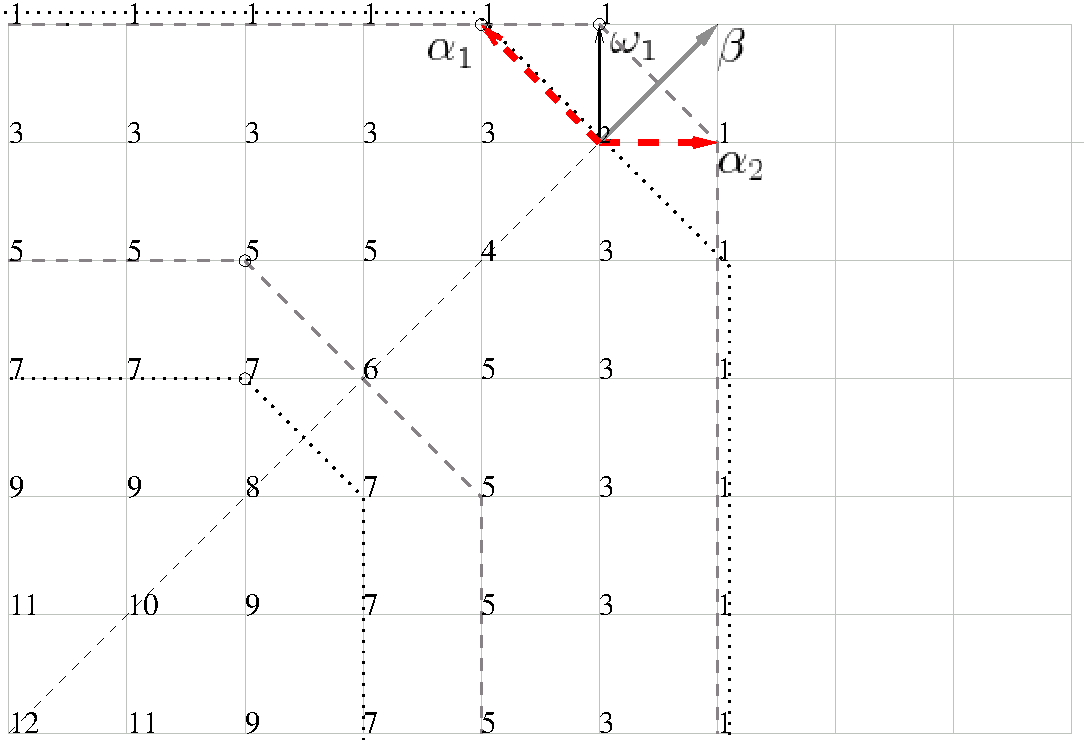
\includegraphics[width=120mm]{B2_Gen_Verma_Decomp.pdf}
  }
  \caption{Generalized Verma modules  for the regular embedding of $A_1$ into $B_2$.
  Simple roots $\alpha_1, \alpha_2$ of $B_2$ are presented as the dashed vectors.
    The simple root $\beta = \alpha_1+2\alpha_2$ of $A_1$ is indicated as the grey vector. The
    decomposition of $L^{\omega_{1}}$ is indicated by
    the set of contours of the involved generalized Verma
  modules. Dashed contours correspond to positive $\epsilon(u)$ and dotted to negative.}

 \label{fig:B2_Verma_Decomp}
\end{figure}

\end{example}

\begin{remark}
As it was proved in \cite{humphreys2008representations} (see Proposition 9.6
) characters of the generalized Verma modules $M_{I}^{\mu _{\frak{a}%
_{\perp }}\left( u\right) }$ can be described as linear combinations of
ordinary Verma modules of $\frak{g}$:
\begin{equation*}
\mathrm{ch}M_{I}^{\mu _{\frak{a}_{\perp }}\left( u\right) }=\sum_{w\in W_{%
\frak{a}_{\perp }}}\epsilon \left( w\right) \mathrm{ch}M^{w\left( \mu _{%
\frak{a}_{\perp }}\left( u\right) +\rho _{\frak{a}_{\perp }}\right) -\rho _{%
\frak{a}_{\perp }}}
\end{equation*}
Substituting this expression in\ (\ref{char in gen verma mod}) and using the
definitions (\ref{mu-a},\ref{mu-a-tilda}) and (\ref{defect ort}) we reconstruct
the standard Weyl-Verma decomposition of the character:
\begin{equation*}
\mathrm{ch}\left( L^{\mu }\right) =\sum_{w\in W}\;\epsilon (u)\mathrm{ch}%
M^{w\left( \mu +\rho \right) -\rho }.
\end{equation*}
\end{remark}

\section{BGG resolution and branching}

In \cite{lepowsky1977generalization} it was demonstrated that for the
highest weight module $L^{\mu }$ with $\mu \in P^{+}$ the sequence

\begin{equation}
0\rightarrow M_{r}^{I}\overset{\delta _{r}}{\rightarrow }M_{r-1}^{I}\overset{%
\delta _{r-1}}{\rightarrow }\ldots \overset{\delta _{1}}{\rightarrow }%
M_{0}^{I}\overset{\varepsilon }{\rightarrow }L^{\mu }\rightarrow 0,
\label{resolution sequence}
\end{equation}
with
\begin{equation}
M_{k}^{I}=\bigoplus_{u\in U,\;\mathrm{length}\left( u\right)
=k}M_{I}^{u\left( \mu +\rho \right) -\rho },\quad M_{0}^{I}=M_{I}^{\mu }
\label{Verma elements sequence}
\end{equation}
(the generalized BGG resolution) is exact and formula (\ref{gen Weyl-Verma}%
) is a cosequence of this resolution.

\begin{figure}[h!bt]
 \noindent\centering{
   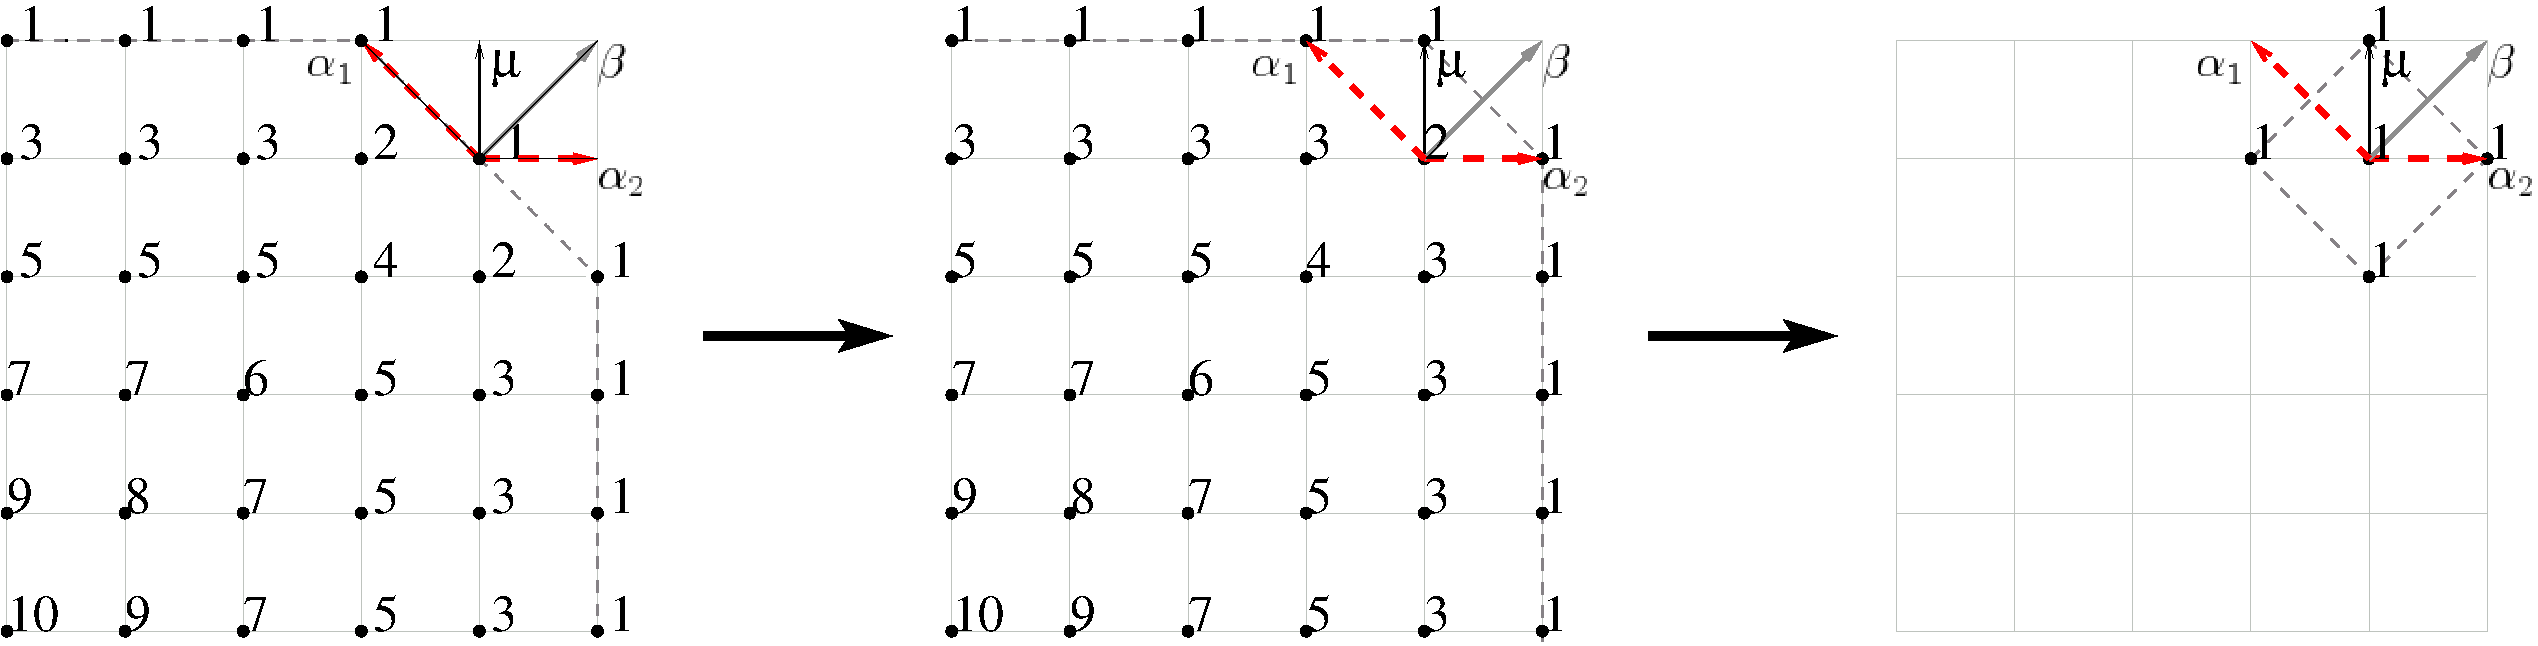
\includegraphics[width=140mm]{B2_Exact.pdf}}
 \caption{Injection $A_1\hookrightarrow B_2$ (see Figure \ref{fig:B2_Verma_Decomp}).
 The orthogonal partner is $A_1$ corresponding to the root $\alpha_1$.
 The resolution of the simple module $L^{\omega_1}$.
 Presented is the central part of the exact sequence
   $0 \to Im(\delta_2) \to \left( e^{\mu _{\widetilde{%
\frak{a}}}\left( e\right) }\mathrm{ch}M_{I}^{\pi _{\afb}\left[ \omega_1 \right] -%
\mathcal{D}_{\afb} }=M^{\omega_1}_{I}\right) \to
   L^{\omega_1}\to 0 $.  Here $\mu _{\widetilde{\frak{a}}}\left( e\right) =\pi _{\aft}\left[ \mu \right] + \mathcal{D}_{\afb}$.
   }
\end{figure}


\begin{statement}

Let $L^{\mu }$ be the highest weight $\frak{g}$-module with $\mu \in P^{+}$
,let its regular subalgebra $\mathfrak{a}_{\bot }\hookrightarrow \frak{g}$
be orthogonal to a reductive subalgebra $\frak{a}\hookrightarrow \frak{g}$.
Then the decomposition (\ref{sing decomp main}) defines both the generalized
resolution of $L^{\mu }$ with respect to $\frak{a}_{\perp }$ and the
branching rules for $L^{\mu }$ with respect to $\frak{a}$ .
\end{statement}

\begin{proof}
Put
\begin{equation*}
\mathrm{ch}M_{I}^{u\left( \mu +\rho \right) -\rho }=e^{\mu _{\widetilde{%
\frak{a}}}\left( u\right) }\mathrm{ch}M_{I}^{\mu _{\frak{a}_{\perp }}\left(
u\right) },\mathrm{ch}M_{I}^{\mu }=e^{\mu _{\widetilde{\frak{a}}}\left(
e\right) }\mathrm{ch}M_{I}^{\pi _{\frak{a}_{\perp }}\left[ \mu \right] -%
\mathcal{D}_{\frak{a}_{\perp }}}
\end{equation*}
with\ $\mu _{\widetilde{\frak{a}}}\left( u\right) ,\mu _{\frak{a}_{\perp
}}\left( u\right) $ and $\mathcal{D}_{\frak{a}_{\perp }}$ as in Lemma \ref{Psi-decomp-lemma} and $%
u\in U$ defined by (\ref{U-def}). This gives the elements of the filtration
sequence (\ref{resolution sequence}).

Consider the set $\left\{ \mu _{\frak{a}_{\perp }}\left( u\right) |u\in
U\right\} $ as the highest weights for the simple modules $L_{\frak{a}%
_{\perp }}^{\mu _{\frak{a}_{\perp }}\left( u\right) }$ and evaluate their
dimensions. Together with
$\left\{ \mu _{\widetilde{\mathfrak{a}}}\left( u\right) |u\in
U\right\} $ this gives the set of singular weights
\begin{equation*}
\left\{ \epsilon (u)\;
e^{\mu _{\widetilde{\mathfrak{a}}}\left( u\right) }
\dim \left( L_{\frak{a}_{\perp }}^{\mu _{\frak{a}_{\perp
}}\left( u\right) }\right) \right\} .
\end{equation*}
The branching $L_{\frak{g}\downarrow \frak{a}}^{\mu }=\bigoplus\limits_{\nu
\in P_{\frak{a}}^{+}}b_{\nu }^{\left( \mu \right) }L_{\frak{a}}^{\nu }$ is
then fixed by the injection fan $\Gamma _{\frak{a}\rightarrow \frak{g}}$ and
the relation (\ref{recurrent rel}). The latter gives us the coefficients $k_{\xi
}^{\left( \mu \right) }$ and thus defines $b_{\nu }^{\left( \mu \right) }$
due to the property $b_{\nu }^{\left( \mu \right) }=k_{\nu }^{\left( \mu
\right) }$ for $\nu \in \overline{C_{\frak{a}}}$ .
\end{proof}

\begin{corollary}

Let $L^{\mu }$ be the highest weight $\frak{g}$-module with $\mu \in P^{+}$
and $\frak{a}\hookrightarrow \frak{g}$ -- a reductive subalgebra in $\frak{g}
$. Let $\frak{a}_{\perp }$, the orthogonal partner for $\frak{a}$, be
equivalent to $A_{1}$, $\frak{a}_{\perp }\approx $ $A_{1}$, and $\widetilde{%
\frak{a}}=\frak{a}\oplus \frak{h}_{\perp }$ with $\frak{h=\frak{h}_{\frak{a}}%
}\oplus \frak{h}_{\frak{a}_{\perp }}\oplus \frak{h}_{\perp }$. Let $L_{%
\frak{g}\downarrow \widetilde{\frak{a}}}^{\mu }=\bigoplus\limits_{\nu \in P_{%
\widetilde{\frak{a}}}^{+}}b_{\nu }^{\left( \mu \right) }L_{\widetilde{\frak{a%
}}}^{\nu }$ be the branching of $L^{\mu }$ with respect to $\widetilde{\frak{%
a}}$. Then the branching coefficients $b_{\nu }^{\left( \mu \right) }$
define the generalized resolution (\ref{resolution sequence}) of $L^{\mu }$
with respect to $\frak{a}_{\perp }$.
\end{corollary}

\begin{proof}
Let $\alpha $ be the simple root of $A_{1}$. Use the Weyl transformations
to identify it with some simple root of $\frak{g}$, say $\alpha _{1}$.
Construct the singular element for the module $L_{\frak{g}\downarrow
\widetilde{\frak{a}}}^{\mu }$, i.e. the $\Psi _{\widetilde{\frak{a}}%
}^{\left( L_{\frak{g}\downarrow \widetilde{\frak{a}}}^{\mu }\right)
}=\sum_{\nu \in P_{\widetilde{\frak{a}}}^{+},b_{\nu }^{\left( \mu \right)
}>0}b_{\nu }^{\left( \mu \right) }\Psi _{\widetilde{\frak{a}}}^{\left( \nu
\right) }$ , and decompose it $\Psi _{\widetilde{\frak{a}}}^{\left( L_{\frak{%
g}\downarrow \widetilde{\frak{a}}}^{\mu }\right) }=k_{\xi }^{\left( \mu
\right) }e^{\xi }$. In our case the representatives $u$ in the
recurrent relation (\ref{recurrent rel}) are uniquely determined by the weight $\xi $:
\begin{equation*}
\epsilon (u\left( \xi \right) )\;\dim \left( L_{\frak{a}_{\perp }}^{\mu _{%
\frak{a}_{\perp }}\left( u\left( \xi \right) \right) }\right) =-s\left(
\gamma _{0}\right) k_{\xi }^{\left( \mu \right) }-\sum_{\gamma \in \Gamma _{%
\widetilde{\frak{a}}\rightarrow \frak{g}}}s\left( \gamma +\gamma _{0}\right)
k_{\xi +\gamma }^{\left( \mu \right) }.
\end{equation*}
We have
\begin{equation*}
\dim \left( L_{\frak{a}_{\perp }}^{\mu _{\frak{a}_{\perp }}\left( u\left(
\xi \right) \right) }\right) =\left| s\left( \gamma _{0}\right) k_{\xi
}^{\left( \mu \right) }+\sum_{\gamma \in \Gamma _{\widetilde{\frak{a}}%
\rightarrow \frak{g}}}s\left( \gamma +\gamma _{0}\right) k_{\xi +\gamma
}^{\left( \mu \right) }\right|
\end{equation*}
and
\begin{equation*}
\mu _{\frak{a}_{\perp }}\left( u\left( \xi \right) \right) =\frac{1}{2}%
\left( \dim \left( L_{A_{1}}^{\mu \left( \xi \right) }\right) -1\right)
\alpha _{1}
\end{equation*}
The set of generalized Verma modules $e^{\xi +\mathcal{D}%
_{\frak{a}_{\perp }}}\mathrm{ch}M_{I}^{\mu _{\frak{a}_{\perp }}\left(
u\left( \xi \right) \right) }$ is thus fixed:
\begin{equation*}
\left\{ e^{\mu _{\widetilde{\mathfrak{a}}}\left( u\right) }\mathrm{ch}%
M_{I}^{\mu _{\frak{a}_{\perp }}\left( u\right) }|u\in U\right\} .
\end{equation*}
Classifying these modules according to the length of $u$
we get the components (\ref{Verma elements sequence}) of the resolution (\ref{resolution sequence}).
\end{proof}



\section{Conclusions}

\label{sec:conclusions}

In \cite{2010arXiv1007.0318L} it was demonstrated that the injection fan
recursive mechanism works also for special injections. It must be mentioned
that in this case the Weyl-Verma decompositions can also be obtained. The
resolutions corresponding to special subalgebras describe the relations
between the projections of characters of the initial module and the generalized
Verma modules with highest weights in the subspace of $h^*$.

Consider the situation where the simple roots are prescribed by some
external factors (originating in physical applications conditions, for
example). In this case the orthogonal partner cannot be generated by simple
root vectors only. The elements $\frak{u}_{I}^{+}:=\sum_{\eta \in \Delta
^{+}\setminus \Delta _{I}^{+}}\frak{g}_{\eta }$ do not form a subalgebra in $%
\mathfrak{g}$ because some nonsimple roots are lost in $\Delta ^{+}\setminus
\Delta _{I}^{+}$. It is important to indicate that in this case the
Weyl-Verma formula still exists. In it the generalized Verma modules
correspond to the contractions \cite{Doebner1967Melsheimer} of the algebra $%
\frak{n}^{+}$ and the Weyl-Verma relations describe the decomposition of
the representation space of $L^{\mu}$ into the set of generalized Verma
modules of contracted algebra $U\left(\frak{n}_c^{+}\right)$. The weight
vectors are formed by the PBW-basis of $U\left(\frak{n}_c^{+}\right)$ and of
$U\left( \mathfrak{a}_{\bot} \right)$. To consider such space as a $%
\mathfrak{g}$-module we must perform the deformation \cite
{Nijenhuis1966Richardson} of the algebra $\frak{n}_c^{+}$ (and thus restore the
initial composition law). The space survives and after such a deformation
the initial algebra generators will act properly on it.

\section{Acknowledgments}

The authors express their sincere gratitude to all those who prepared and
performed the III International Conference "Models in Quantum Field Theory -
2010" dedicated to 70-th anniversary of A. N. Vassiliev.

The work was supported in part by the RFFI grant N 09-01-00504 and by the Chebyshev Laboratory
(Department of Mathematics and Mechanics, Saint-Petersburg State
University) under the grant 11.G34.31.2006 of the Government of the
Russian Federation.


\bibliographystyle{plain}
\bibliography{article-ru}
{}

\end{document}
